\documentclass[11pt]{article}
\usepackage[margin=1in]{geometry}
\usepackage{booktabs}
\usepackage{graphicx}
\usepackage{longtable}
\usepackage{array}
\usepackage{xcolor}
\usepackage{hyperref}

\title{Segmentation Evaluation Report for Magnaporthe Growth Analysis}
\author{evaluation\_report pipeline}
\date{\today}

\begin{document}
\maketitle

\section{Introduction}
This report validates a hybrid segmentation system for Magnaporthe growth analysis on 22 matched annotation pairs out of 24 available predictions. The goal is to quantify how closely the final predicted segmentation contour matches the ground-truth annotation set.

\section{Methods}
\subsection{Hybrid segmentation pipeline}
The evaluated output is the final hybrid segmentation contour produced after classical segmentation, U-Net support, Gemma-guided decision logic when available, and SAM refinement. Ground-truth and prediction masks are compared directly as binary foreground maps.

\subsection{Evaluation protocol}
Each predicted annotation is matched to a ground-truth annotation by normalized filename stem. The polygons are rasterized into binary masks, aligned to a shared canvas when needed, and then evaluated pixel-wise. The dataset-level summary reports the mean, standard deviation, and bootstrap confidence interval of each metric.

\section{Metric definitions}
Let $TP$, $FP$, and $FN$ denote true-positive, false-positive, and false-negative pixel counts.

\[
\mathrm{Precision} = \frac{TP}{TP + FP}
\]

\[
\mathrm{Recall} = \frac{TP}{TP + FN}
\]

\[
F_1 = \frac{2 \cdot \mathrm{Precision} \cdot \mathrm{Recall}}{\mathrm{Precision} + \mathrm{Recall}}
\]

\[
\mathrm{IoU} = \frac{TP}{TP + FP + FN}
\]

\section{Results}
\subsection{Aggregate metrics}
\begin{center}
\begin{tabular}{lrrrr}
\toprule
Metric & Mean & Std & CI lower & CI upper \\
\midrule
precision & 0.7272 & 0.2345 & 0.6254 & 0.8204 \\
recall & 0.9133 & 0.2160 & 0.8104 & 0.9789 \\
f1\_score & 0.7988 & 0.2096 & 0.7020 & 0.8723 \\
iou & 0.7019 & 0.2298 & 0.6011 & 0.7911 \\
\\
\bottomrule
\end{tabular}
\end{center}

\subsection{Headline values}
\begin{itemize}
\item Mean precision: 0.7272
\item Mean recall: 0.9133
\item Mean F1-score: 0.7988
\item Mean IoU: 0.7019
\item Missing prediction-to-GT matches: 2
\end{itemize}

\subsection{Area agreement statistics}
\begin{center}
\begin{tabular}{lr}
\toprule
Statistic & Value \\
\midrule
Mean predicted area (px) & 467628.2727 \\
Mean GT area (px) & 405068.5455 \\
Mean relative area error (\%) & 38.0582 \\
Median relative area error (\%) & 30.3602 \\
Shape alignment rate & 0.7273 \\
\\
\bottomrule
\end{tabular}
\end{center}

\subsection{Figures}
\begin{figure}[h!]
\centering
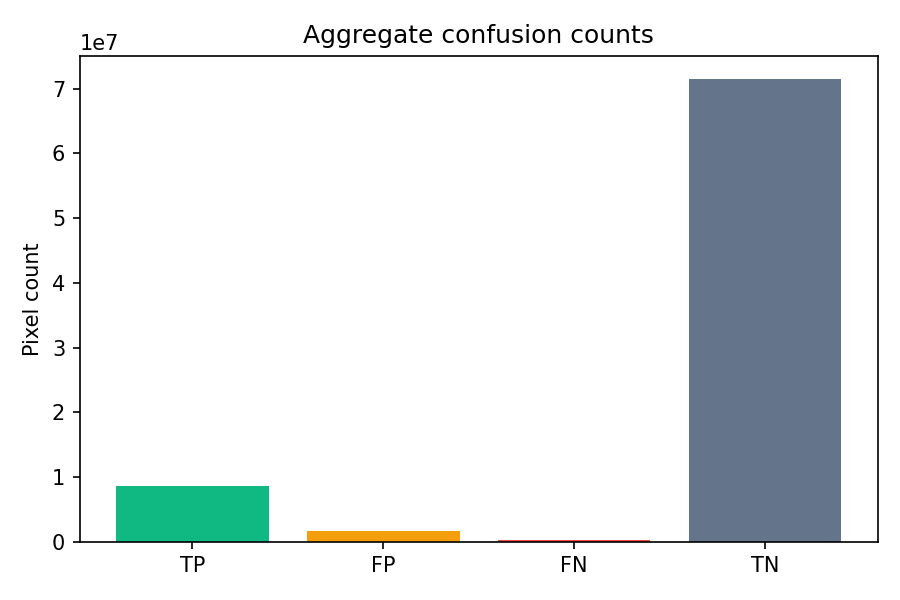
\includegraphics[width=0.7\textwidth]{figures/confusion_counts.png}
\caption{Aggregate confusion counts across the evaluation dataset.}
\end{figure}

\begin{figure}[h!]
\centering
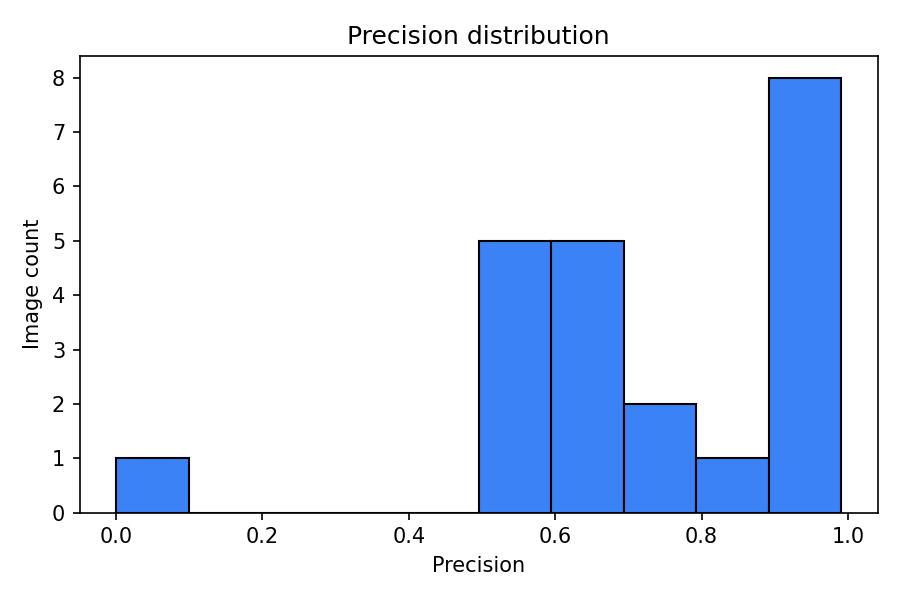
\includegraphics[width=0.48\textwidth]{figures/precision_histogram.png}
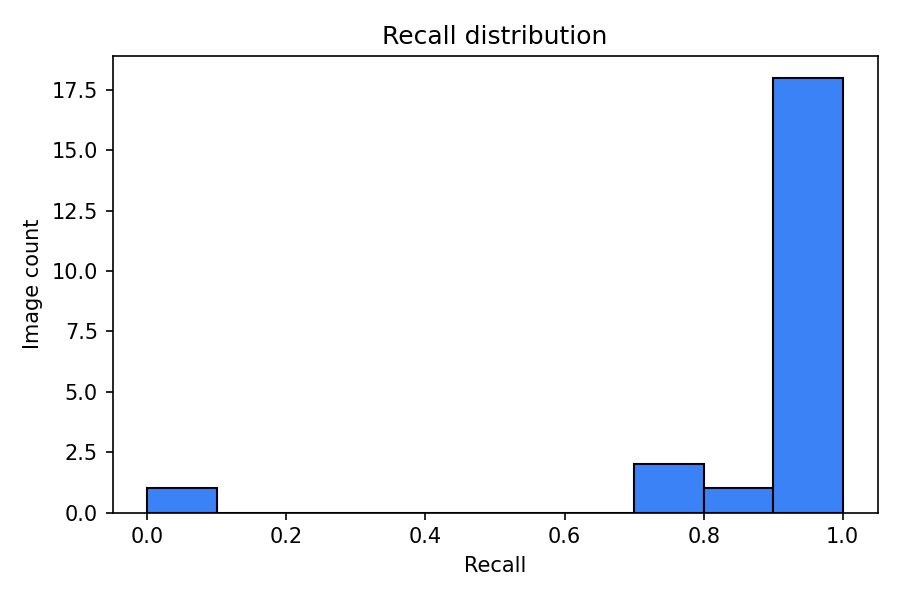
\includegraphics[width=0.48\textwidth]{figures/recall_histogram.png}
\caption{Precision and recall distributions.}
\end{figure}

\begin{figure}[h!]
\centering
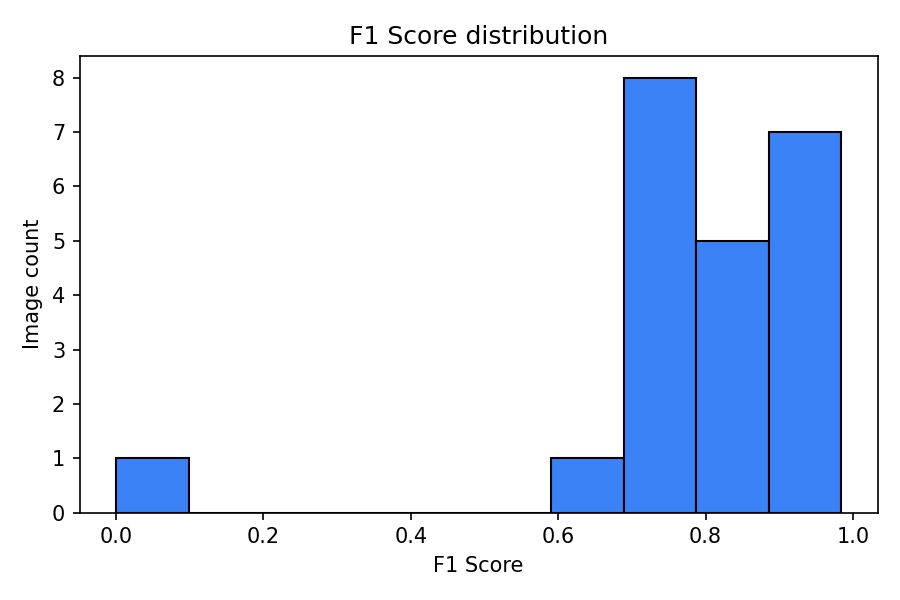
\includegraphics[width=0.48\textwidth]{figures/f1_score_histogram.png}
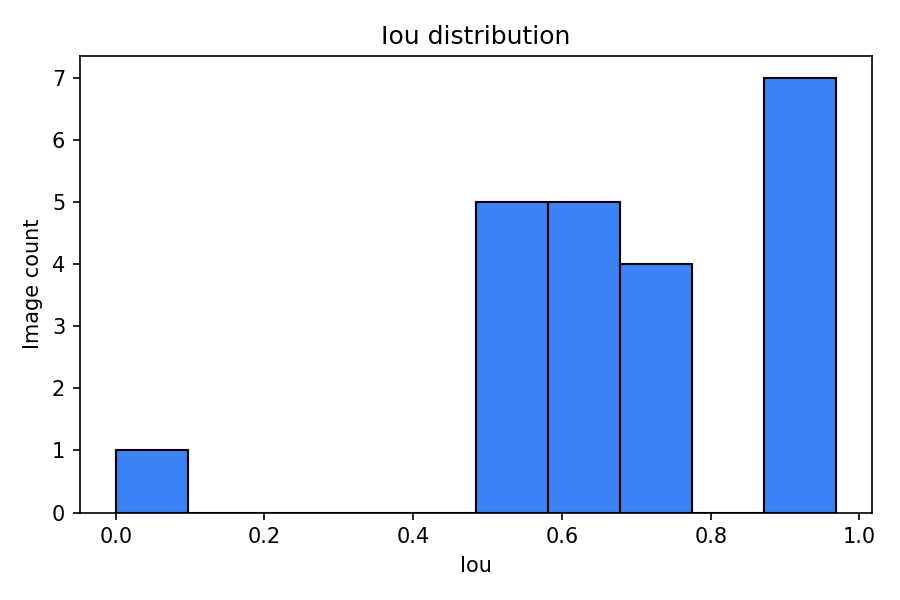
\includegraphics[width=0.48\textwidth]{figures/iou_histogram.png}
\caption{F1-score and IoU distributions.}
\end{figure}

\begin{figure}[h!]
\centering
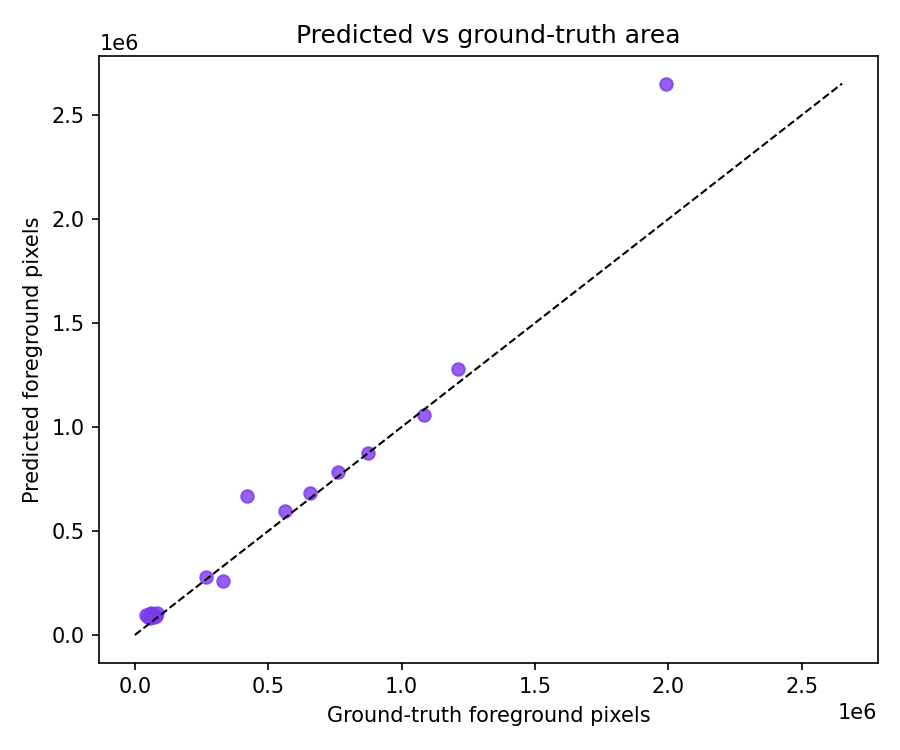
\includegraphics[width=0.48\textwidth]{figures/area_agreement.png}
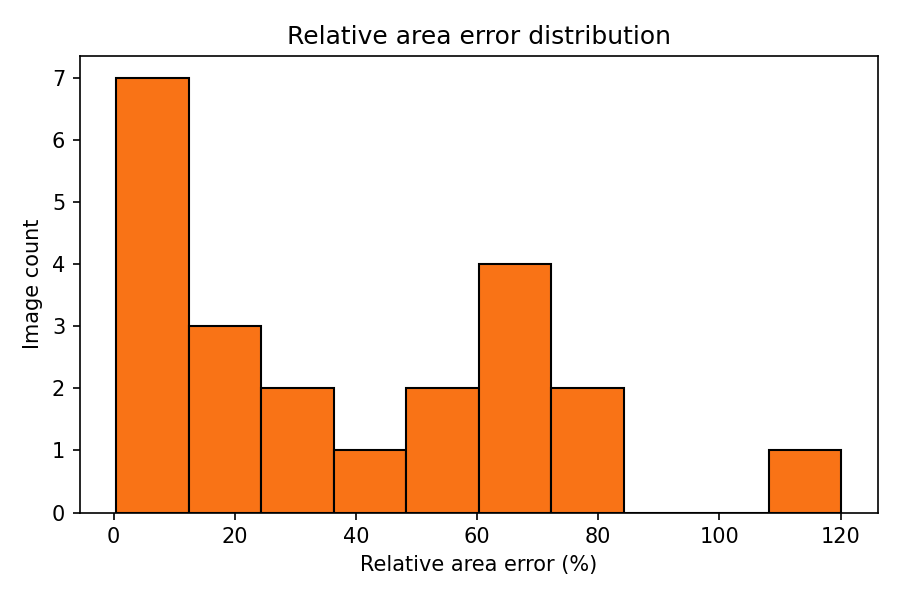
\includegraphics[width=0.48\textwidth]{figures/relative_area_error_histogram.png}
\caption{Annotation-derived area agreement and relative area error.}
\end{figure}

\section{Discussion}
The results summarize how well the final hybrid segmentation output aligns with manual ground truth on the available annotation set. Precision reflects over-segmentation control, recall reflects missed-colony risk, F1 balances both, and IoU gives a compact overlap-based score. Bootstrap confidence intervals provide a small-sample uncertainty estimate rather than a single optimistic point value.

\subsection{Conclusions}
Across 22 matched mask pairs out of 24 available predictions, the hybrid segmentation pipeline delivered moderate overlap with the manual labels. The mean IoU was 0.7019 with a bootstrap 95\textbackslash{}\% confidence interval of [0.6011, 0.7911], while the mean F1-score was 0.7988. Precision (0.7272) and recall (0.9133) show whether the system leans more toward under-segmentation or over-segmentation. The median relative foreground-area error was 30.36\textbackslash{}\%, and 0.7273 of pairs required canvas-size alignment before pixel-wise comparison. These statistics suggest that the final performance estimate is driven by the full annotation set rather than a single optimistic example, but the unmatched files and the alignment rate should still be reviewed before treating the numbers as a final benchmark.

\end{document}
